\section{Transparent Acceleration}
\label{sec_transacc}


Transparent acceleration of workloads is one of the design goals of
the {\em Transformer}. Transparent acceleration refers to the speedup of
an application using hardware accelerators without the need for source
code access, recompilation, or user intervention at run-time. We argue that such a feature is one of
the most important factors that enables the practical deployment of the
proposed heterogeneous architecture for the following reasons. 
First, the users'
workloads are typically present in the form of binary executables. The difficulties in obtaining access to the source code as well as 
rewriting the application impose tremendous obstacles for taking
advantage of the hardware accelerator. Second, the development environment
for user applications cannot be easily duplicated or emulated within
the run-time environment due to the complexity and variety of
the compilers as well as the libraries. As a result, the recompilation of an
application for hardware acceleration is either infeasible or
problematic. Third, recompilation of user applications introduces
delays which are often unnecessary and/or intolerable. Therefore
transparent acceleration is critical when applying hardware accelerators to unpredictable
workloads.

In order to achieve transparent acceleration and ease the work of programmers,
we focus on the acceleration of commonly used libraries such as
libopenssl. Such libraries are made available with well known APIs for
their core functions, and are often the targets of acceleration. For
example, 3DES, a classic block cipher, is one of the many functions
contained within libopenssl, which also includes a cryptography library implementing the Secure
Sockets Layer (SSL) as well as the Transport Layer Security
(TLS)\cite{wikissl} protocols. By taking on the form of a dynamically linked
library, libopenssl provides entry points for its functions, including
3DES. We propose to add a layer of wrapper functions that profile and
intercept the calls from user applications to the libraries, which can then
be accelerated through the use of programmable logic. 


\begin{figure}
    \centering
    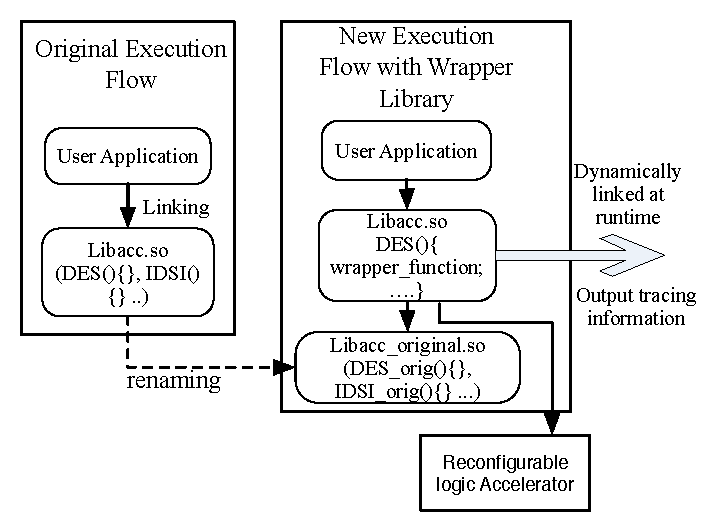
\includegraphics[width=4.0 in]{HPCA14-wrapperlib}
    \caption{Original and Modified Execution Flow}
    \label{fig_transacc_flow}
\end{figure}

Wrapper functions are presented in the form of dynamically linked
libraries, which utilize renaming in order to replace the original libraries. As a result,
the calls to the original dynamic library are directed to the wrapper
functions due to the linker stub \cite{linkerstub}. The modified
execution flow is shown in Figure \ref{fig_transacc_flow}.  The
original dynamically linked library is renamed by adding a suffix
{\em ``\_original''}.  The dynamically linked library functions are renamed by rewriting the corresponding symbol table. 
We create our new dynamic-linked library with the same name as the original library, and
incorporate a wrapper function to intercept all the library calls, specifically calls to the original function names, and
redirect them to either the original software library or the hardware
accelerator. As 
Section \ref{sec_perf} demonstrates, the wrapper library is
executed on a CPU core with a very small amount of overhead.

The responsibilities of the wrapper functions are two fold.
First, with regards to {\em profiling},
a wrapper library records the number of calls to each of the
library functions. Such counters reflect the demands on individual
functions, for example 3DES, which are used by the reconfiguration
controller to determine which functions are to be accelerated within the
programmable hardware. We provide details regarding the algorithms for the
run-time reconfiguration in Section \ref{sec_runtime_reconfig}.
Second, with regards to {\em function call redirection},
 a wrapper function directs the
execution flow to an appropriate path, either allowing the continuation of software instruction execution on a core or
accelerating software instruction execution within a programmable hardware unit. The wrapper functions
are aware of the currently accelerated functions on the programmable
accelerators, and such knowledge is updated by the reconfiguration
controller. If the required function is currently supported in the hardware
accelerator, this call and subsequent ones to the particular library
function(s) are redirected to the accelerator, thus reducing execution
time.

Library based transparent acceleration benefits dynamically
linked applications which are well supported in modern operating
systems, such as Windows and Linux. For statically linked applications,
although the dynamic library based transparent acceleration is limited
in detecting library calls and redirecting instruction flow to
hardware accelerators, we argue that such limitations are not inherent
within the context of the proposed heterogeneous architecture. A user can still
incorporate our wrapper functions into their applications so that any 
calls to compute-intensive functions will be appropriately instrumented.  Furthermore,
subsequent function calls are redirected to programmable accelerators after the
run-time system determines that the function should be sped
up with a hardware based accelerator.
We illustrate the process of a sample acceleration function call in Algorithm \ref{alg_sample_func}.

\begin{algorithm}[htb]
\scriptsize
\caption{Sample Acceleration Function Call}
\label{alg_sample_func}
\begin{algorithmic}[1]
\STATE {\em In User Function:}
\STATE {Call: DES (arg1, arg2, arg3) \newline}
\STATE {\em In Wrapper Function DES(arg1, arg2, arg3):}

\IF {DES is called}
	\STATE {RequestCounter ++ \COMMENT{Increase Request Counter by 1}}
	\IF {Request tracking time window is finished}
		\STATE{$D_{x} = \sum_{i=1}^{H}C(x,i)$ \COMMENT{Total demand}}
		\STATE{$DC_{x} = \sum_{i=1}^{H-1}(|C(x, i+1)-C(x, i)|)$\COMMENT{Demand changes}}
		\IF {Use naive scheduling}
			\STATE{$P_x = a \times D_x + (1-a) \times DC_x$ \COMMENT{Priority of this function}}
		\ENDIF
		\IF {Use Bandwidth/Speedup First scheduling}
			\STATE{$P_x = $ the result of 2D-knapsack combination}
		\ENDIF
	\ENDIF
	\IF {Function DES meets the requirement of being scheduled}
		\STATE{$ConfigStart \leftarrow 1$; $AccType \leftarrow 0$ \COMMENT{3DES is type 0}}
		\STATE {$ArgNum \leftarrow 3$; $AccPtr \leftarrow \& arg1$; $DS \leftarrow 1$}
		\IF {$ConfigDone = 1\quad\AND\quad DD = 1$}
			\STATE{$AccStart \leftarrow 1$}
		\ENDIF
		\IF {$AccDone = 1$}
			\STATE{Get back to previous thread.}
		\ENDIF
	\ELSE
		\RETURN $DES(arg1, arg2, arg3) \COMMENT{\text{Software  Version}}$
	\ENDIF
\ENDIF

\end{algorithmic}

\end{algorithm}








